\section{Results}
\begin{itemize}
\item Property of the graph (number of components, node per component)

\item For each scenario we vary the number of threads and partitions. 

\item For each scenario we compute the loss. 

\item Scalability - Replicate the graph:
\end{itemize}

\begin{figure}
\centering
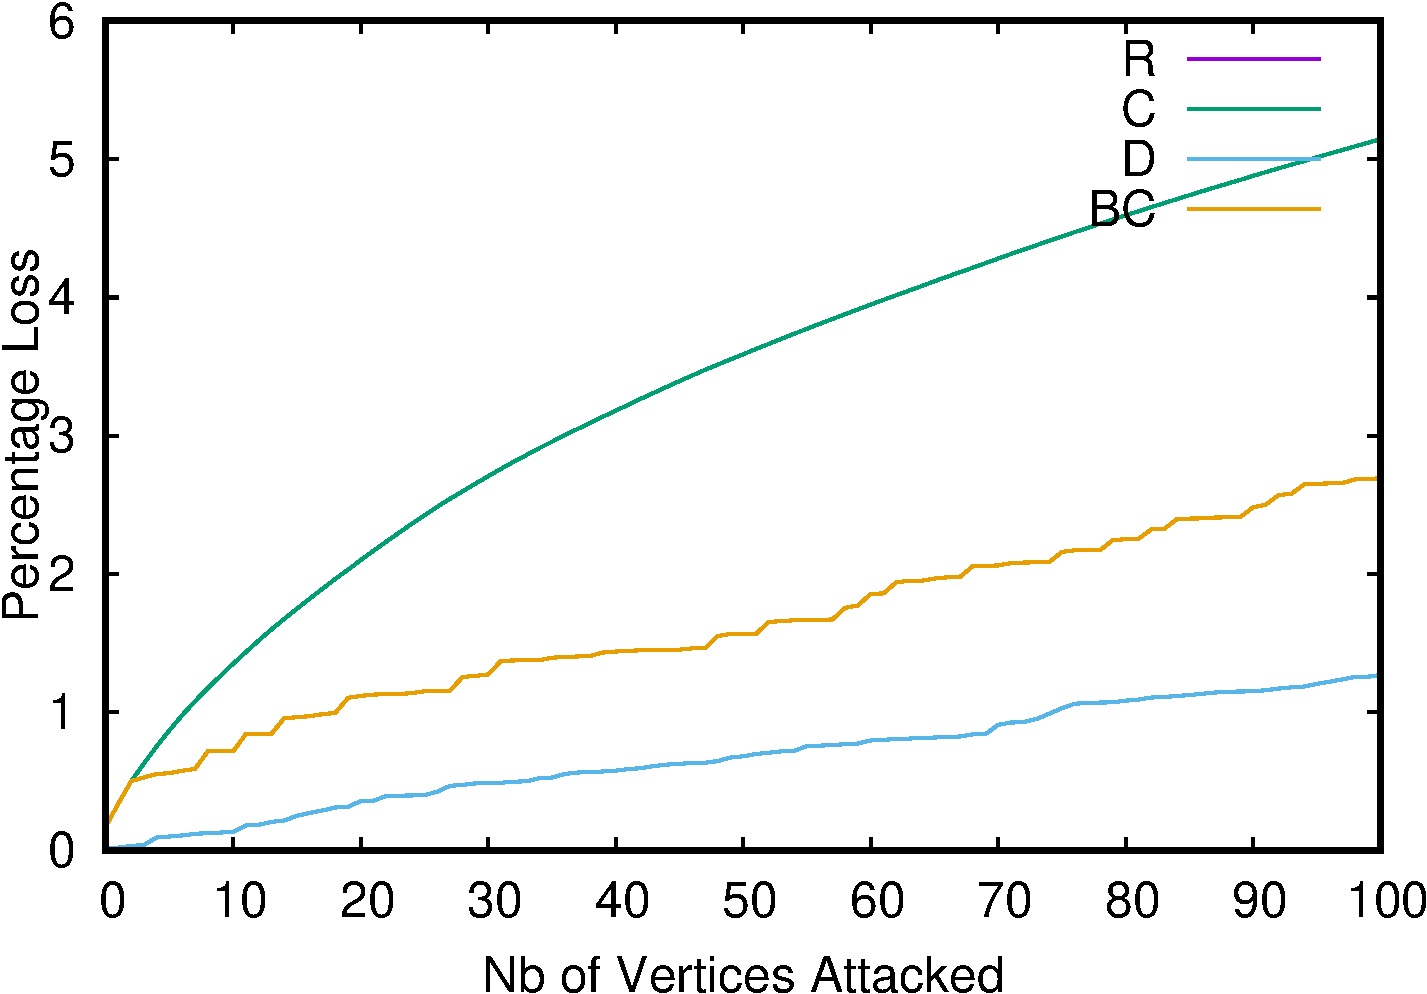
\includegraphics[scale=0.35]{bench/loss-100-crop.pdf}
\label{fig:loss-100}
\caption{Loss first 100. todo}
\end{figure}

\begin{figure}
\centering
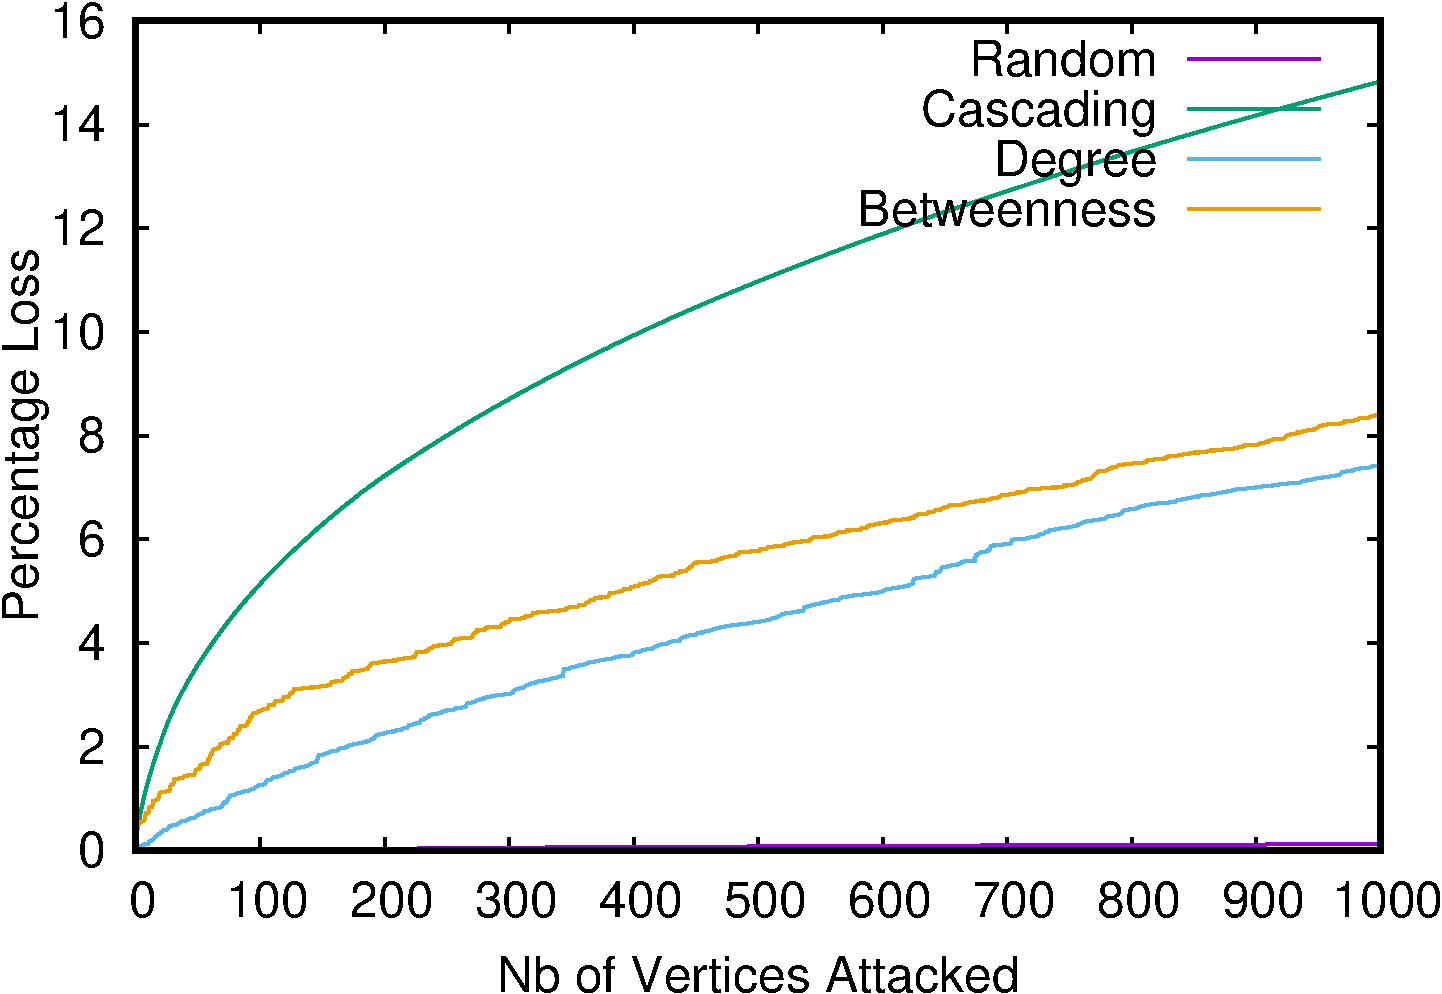
\includegraphics[scale=0.35]{bench/loss-1000-crop.pdf}
\label{fig:loss-1000}
\caption{Loss first 1000.. todo}
\end{figure}

\begin{figure}
\centering
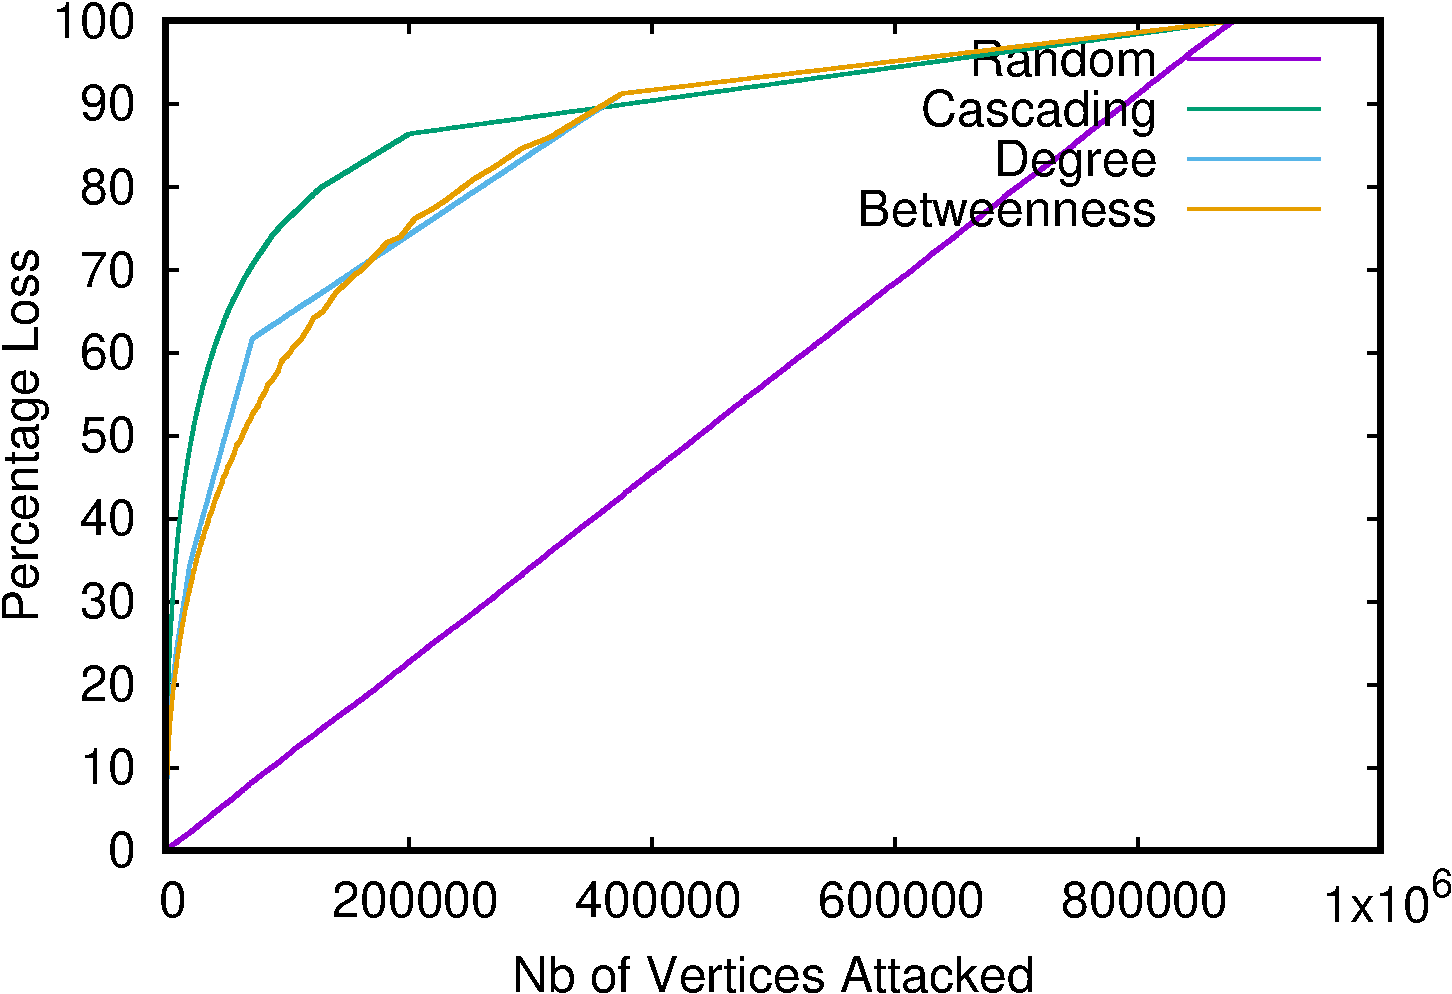
\includegraphics[scale=0.35]{bench/loss-all-crop.pdf}
\label{fig:loss-100}
\caption{Loss all... to do}
\end{figure}


\onecolumngrid
\begin{table*}
\label{tab:graph1}
\caption{graph1.. todo}
{\small
\begin{tabular}{||c||c|c|c|c||c|c|c|c||c|c|c|c||c|c|c|c|}
\hline
\textbf{Threads}	&\cellcolor{black!10}BC-4&	\cellcolor{black!10}BC-8	&\cellcolor{black!10}BC-16	&\cellcolor{black!10}BC-32&	\cellcolor{black!10}C-4	&\cellcolor{black!10}C-8&	\cellcolor{black!10}C-16&	\cellcolor{black!10}C-32&	\cellcolor{black!10}D-4&	\cellcolor{black!10}D-8	&\cellcolor{black!10}D-16&\cellcolor{black!10}	D-32&	\cellcolor{black!10}R-4	&\cellcolor{black!10}R-8&	\cellcolor{black!10}R-16&	\cellcolor{black!10}R-32 \\ \hline \hline
64&		27	&17	&22	&41	&53	&34	&32	&52	&26	&15	&20	&41	&23	&17	&20	&39			\\ \hline					
32&		24	&17	&19	&37	&52	&33	&31	&49	&20	&16	&18	&36	&20	&19	&19	&36	\\ \hline
16&		24	&18	&22	&39	&53	&35	&37	&54	&21	&16	&19	&37	&19	&16	&20&37	\\ \hline
8	&	25	&25	&30	&54	&55	&50	&56	&80	&21	&21	&26	&51	&20	&20	&26	&50	\\ \hline
4	&	41	&41	&53	&97	&87	&86	&98	&138	&33	&33	&45	&89	&30	&31	&44	&90	\\ \hline
2&		82	&84	&108	&206	&165	&165	&189	&287	&65	&66	&92	&188	&55	&62	&87	&186	\\ \hline
1&		161	&167	&219	&423	&312	&320	&369	&543	&124	&127	&187	&384	&104	&114	&174	&344	\\ \hline
\end{tabular}
}
\end{table*}
%
\begin{table*}
\label{tab:graph2}
\caption{graph 2.. todo}
{\small
\begin{tabular}{||c||c|c|c|c||c|c|c|c||c|c|c|c||c|c|c|c|}
\hline
\textbf{Threads}	&\cellcolor{black!10}BC-4&	\cellcolor{black!10}BC-8	&\cellcolor{black!10}BC-16	&\cellcolor{black!10}BC-32&	\cellcolor{black!10}C-4	&\cellcolor{black!10}C-8&	\cellcolor{black!10}C-16&	\cellcolor{black!10}C-32&	\cellcolor{black!10}D-4&	\cellcolor{black!10}D-8	&\cellcolor{black!10}D-16&\cellcolor{black!10}	D-32&	\cellcolor{black!10}R-4	&\cellcolor{black!10}R-8&	\cellcolor{black!10}R-16&	\cellcolor{black!10}R-32 \\ \hline \hline
64		&127	&71	&48	&55	&119	&64	&60	&76	&108	&58	&45	&53	&45	&32	&31	&50		 \\ \hline		
32		&120	&59	&45	&49	&116	&68	&56	&71	&108	&57	&42	&47	&40	&29	&29	&45		 \\ \hline			
16		&128	&66	&39	&52	&115	&66	&65	&79	&112	&57	&36	&50	&41	&33	&30	&46 \\ \hline				
8		&123	&66	&56	&77	&120	&97	&98	&121	&106	&54	&46	&68	&40	&34	&39	&63	 \\ \hline			
4		&164	&104	&101	&142	&210	&191	&185	&223	&134	&83	&80	&119	&60	&57	&69	&113	 \\ \hline			
2		&263	&203	&207	&292	&416	&353	&366	&462	&209	&159	&153	&239	&111	&110	&131	&224	 \\ \hline		
1		&452&357	&371	&525	&761	&804	&793	&969	&355	&281	&286	&434	&196	&201	&230	&402 \\ \hline		
\end{tabular}
}
\end{table*}
%
\begin{table*}
\label{tab:graph4}
\caption{graph 4.. todo}
{\small
\begin{tabular}{||c||c|c|c|c||c|c|c|c||c|c|c|c||c|c|c|c|}
\hline
\textbf{Threads}	&\cellcolor{black!10}BC-4&	\cellcolor{black!10}BC-8	&\cellcolor{black!10}BC-16	&\cellcolor{black!10}BC-32&	\cellcolor{black!10}C-4	&\cellcolor{black!10}C-8&	\cellcolor{black!10}C-16&	\cellcolor{black!10}C-32&	\cellcolor{black!10}D-4&	\cellcolor{black!10}D-8	&\cellcolor{black!10}D-16&\cellcolor{black!10}	D-32&	\cellcolor{black!10}R-4	&\cellcolor{black!10}R-8&	\cellcolor{black!10}R-16&	\cellcolor{black!10}R-32 \\ \hline \hline
64 &		525&	317	&171&	117	&411	&179&	127	&123	&430	&220	&134	&104&	133&	79&	70	&87	 \\ \hline		
32	&	491&	274	&153	&99	&387	&202	&123	&121 &449	&243&	149&	100	&122	&101&	64&	75\\ \hline
16	&	473	&311	&133	&96	&401	&184	&127	&137 &457	&236	&113	&77	&130	&86	&62	&78 \\ \hline
8	&	557&	250	&132	&126	&387	&234	&204	&212 &452	&222	&113	&105	&119&	93	&75	&93 \\ \hline
4		&750&	333	&221	&234	&612	&431	&374	&398 &601	&274 &168	&190	&151	&126&	120	&163 \\ \hline
2		&1041 &526 &430 &467	&1042	&791	&736	&793 &888	&436	&344	&395	&273	&235	&237	&337 \\ \hline
1		&1626&902&879 &1021 &2156 &1784 &1577 &1754 &1584 &905 &730 &783& 533 &458 &456 &647 \\ \hline
\end{tabular}
}
\end{table*}
\twocolumngrid

